\chapter{EVENT IDENTIFICATION}
 \label{chap:eventrec}
 \section{Introduction}
Visual event identification has been observed as a potential area of research in several applications like  content-based video retrieval, human computer interaction, etc..  In general, the visual event identification is always modelled as a stochastic temporal processes in the semantic space.  The motivation behind this is to capture the dynamic patterns of event through collective evolution of the semantic concept.  One of the most familiar methods that use this approach is that of Hidden Markov Model (HMM), which has been a favourite for sequential pattern recognition.  However, the HMMs have struggled to incorporate both the spatial and temporal context present in the event.  
\par In another approach by ~\cite{YanKe05}, the event is treated as a space-time volume in the video sequence.  Volumetric features based on optical flow are extracted for event detection.  These are generally used for videos having only single moving object (human) and action.  For complex activity recognition \citep{YanKe07}, the internet videos are already temporarily localized and they focus on identifying the primitive event.
\par A common approach for video classification ~\citep{Liu09}~\citep{Niebles10} involves : extracting local region level features, combining features to fixed size video level description and training a classifier on the features to predict the class labels.  But in these approaches, feature extraction plays a crucial role, and features must be recomputed again for different videos.  Convolutional Neural Network (CNN) replace all three stages with a single neural network ~\cite{Ji13},  and is trained end-to-end from the raw pixel values to classifier outputs. However, CNNs were observed to be computationally expenisve and took longer training periods to effectively optimize the solution.  With the improvements on GPU hardware, CNNs could be scaled to train networks of millions of parameters.

\par Section \ref{sec:cnn} outlines the overall framework of CNNs and discusses the reasons for choosing it for the event identification task over the existing techniques.  Then, we will elaborate the architecture and features supported by the indigenous deep neural network tool kit designed in python in Section \ref{sec:pyDNN}. 

\section{Convolutional Neural Network (CNN)}
 \label{sec:cnn}
 \par Convolutional neural networks (CNN) are a variant of multi-layer perceptron (MLP) that are designed by studying the complex arrangement of cells in the cat's visual cortex.  It comprises of one or more convolutional layers (often with a sub-sampling step), followed by one or more standard MLPs.  There are different varieties of CNN based on the dimensionality of input and convolution operator like CNN-2D, CNN-3D etc.  Figure \ref{fig:cnnarchitecture} depicts a sample CNN architecture with two convolution and subsampling layers followed by a single MLP layer.
 
\begin{figure}[htpb]
   \begin{center}
   		{%
			\setlength{\fboxsep}{5pt}%
			%\setlength{\fboxrule}{1pt}%
	    		\fbox{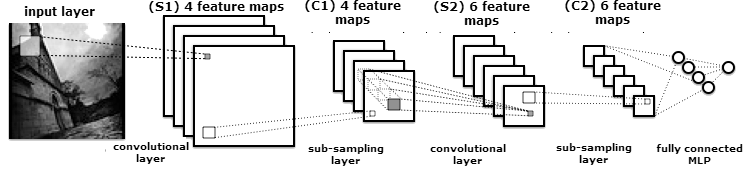
\includegraphics[width=0.98\textwidth]{snaps/cnn.png}}  
	    }%
     \caption[] {A sample CNN architecture \footnotemark}
	\label{fig:cnnarchitecture}  
   \end{center}
 \end{figure} 
\par A major advantage of having CNN is that it learns faster (fewer parameters) compared to MLP with the same number of hidden units.  CNN  also uses gradient based optimization to compute the parameters of the model.  It has been shown that CNNs fits very well onto the visual recognition domain, as it handles very high dimensional data, exploits the topology of image or video, and is invariant to small translation and illumination changes.  CNN leverages the following concepts to tackle the above mentioned challenges:
\footnotetext{\url{http://deeplearning.net/tutorial/lenet.html}}
\subsection{Local Connectivity}
It exploits the spatially local correlation, allowing only local connectivity between neurons of adjacent layers.  Hence, every hidden unit is only sensitive to a small block in the visual field called the receptive field. This drastically reduces the number of connections between the input and the hidden layer which therefore diminishes the number of parameters needed to train the model.
\subsection{Shared Filters}
The hidden units are associated to the receptive field by filters which are shared within a feature map. These filters capture edge like patterns within the receptive field.  Additionally, sharing filters increases the learning efficiency by greatly reducing the number of free parameters to be learned.  Apart from reducing parameters, they extract the same feature at every position, which makes every feature map to be equi-variant to any changes in the input.  The shared filters are associated to the receptive field by a dot product operation which can be expressed as a discrete convolution operation.
\subsection{Pooling/Sub-sampling Hidden Units}
The sub-sampling layer pools the hidden unit output in the non-overlapping neighbourhood.  Pooling can be either average or maximum.  The max-pooling provides local translation invariance and is commonly used.  Pooling also reduces the inputs to the next layer of feature extraction.  With pooling, the feature maps in the latter layer extract coarser features.

\par All these concepts empower CNNs to achieve better generalization in vision problems.  Stacking multiple such layers is a very common approach to attain better responsiveness over a larger visual field.  Some architectural tricks such as rectification and contrast normalization are tried for improving result on large dataset.  The unsupervised pre-training of each filter weight has helped enhance the robustness of the models built.

\section{Python-DNN Toolkit}
\label{sec:pyDNN}
Neural networks can be best implemented using a modular, object-oriented approach,  Where each of the models (DNN, SdA, CNN) are implemented as different classes with member functions performing pre-training (an unsupervised learning), fine-tuning (supervised learning), testing , loading and saving the model.  This approach enables reuse of the code for most of the network models.  Even though the most of the existing toolkits are quite sophisticated, these toolkits are reasonably hard to configure. They needed to be configured either through the command line or by providing the necessary arguments to a function.  Since neural networks take too many parameters, it gets difficult to understand the purpose of any given parameter.  Hence, the \textit{Python-DNN} toolkit was developed.  
\subsection{Architecture}
The toolkit was implemented in python using the numerical computation library named \textit{Theano} \citep{theano}.  It provides a platform to run our toolkit efficiently in both CPU and GPU architecture.  Architecture of the indigenous DNN toolkit is shown on \ref{fig:architecture}.
\begin{figure}[htpb]
   \begin{center}
   		{%
			\setlength{\fboxsep}{5pt}%
			%\setlength{\fboxrule}{1pt}%
	    		\fbox{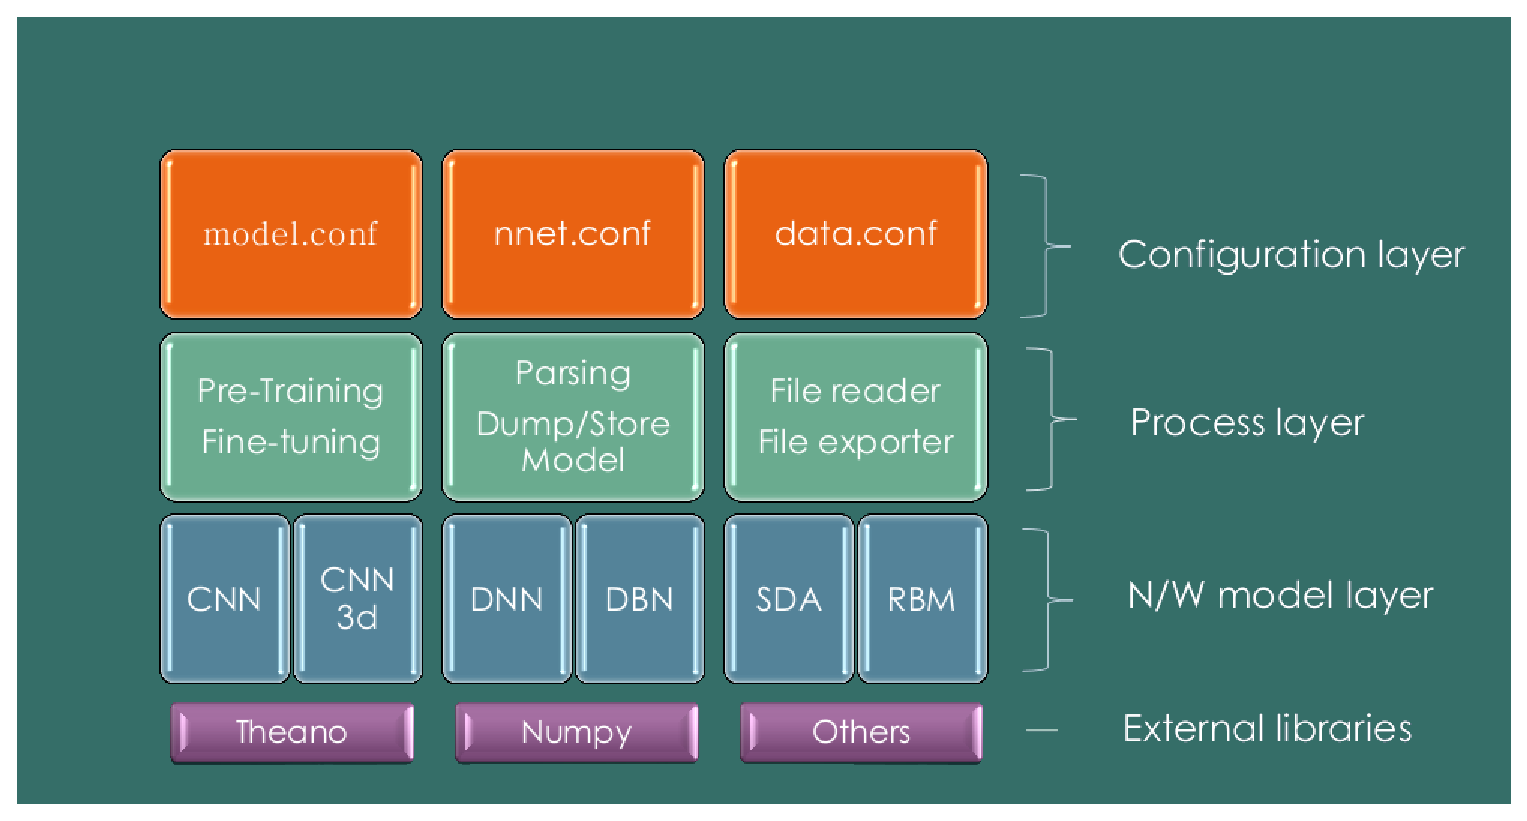
\includegraphics[width=0.90\textwidth]{snaps/colorarchitecture.eps}}  
	    }%
     \caption {Python-DNN architecture}
	 \label{fig:architecture}
   \end{center}
 \end{figure}
Toolkit has been split into four layers : external libraries that include all the dependent libraries, a network model layer that encompass different supervised and unsupervised models supported, a processing layer which focusses on the different operations supported by the different models and the topmost layer configuration layer is the input to the model.  The configuration layer contains three main configurations : 
 \begin{itemize}
	\item {\textbf{model.conf :} it constitute type of model, input model, output model, batch-size, number of outputs(classes), learning rate, momentum and more}
	\item {\textbf{nnet.conf :} it defines a neural network model like number of layers, number of nodes per layer, activation function}
	\item {\textbf{model.conf :} it constitutes a type of model, input model, output model, batch-size, number of outputs(classes), learning rate, momentum and more}
 \end{itemize}
The fine-tuning operation corresponds to the normal back propagation algorithm while the pre-training corresponds to greedy layer-wise learning.  This unsupervised learning at each layer in a way preserves information from the input and disentangles factors of variation.  Sample configurations for some well known datasets like MNIST and CIFAR are also made available with it.
\subsection{Salient Features}
\begin{itemize}
	\item Allows easy configuration of the model, configurations are organized in JSON format thus making the configuration legible to humans.
	\item Supports several types of data readers/writers. 
	\item Enables us to dump bottleneck features for their use in other applications.
	\item Incorporates activation functions : tanh, sigmoid, relu, cappedrelu
	\item Includes drop-out and regularization to tackle over fitting.
	\item Facilitates in loading pre-trained model and dumping the trained model.
	\item Encompass two and three dimensional convolutional models.
	\item Supports pre-training through stacked denoising autoencoders (SdA) and restricted boltzman machine (RBM).
	\item Runs efficiently in CPU and GPU architectures.	
\end{itemize}
Our implementation is publicly made available in github\footnote{\url{https://github.com/IITM-DONLAB/python-dnn}}.  Further details about the the toolkit like installation, configuration and its usage is explained in Appendix \ref{app:pydnn}. This toolkit was built together with Abil N George.
\clearpage

\section{Summary}
The CNN is versatile and yet conceptually simple, and has been adapted for a wide spectrum of cognitive tasks.  It takes advantage of the 2D/3D structure of an input image (or spectrogram in the case of speech signal) by using local connections and shared weights and provides for translational invariance by sub-sampling the layer outputs.  The ready-to-use indigenous toolkit supporting CNN helps in performing the experiments for event identification with ease.  In the next chapter, the experiments on different techniques for the event recognition will be elaborated.